\documentclass[10pt,utf8]{beamer}

\mode<presentation> {
%  \usetheme{Boadilla}
  \usetheme{Madrid}
%	\usetheme{Fzu}
  \setbeamercovered{transparent}
}

\usepackage{palatino}
\usepackage{graphicx}
\usepackage{array}
\usepackage{color}
\usepackage{subfigure}
\usepackage{colortbl}
\usepackage{amsmath}
\usepackage{hyperref}
\usepackage{listings}
\usepackage{fancyvrb}
\usepackage[export]{adjustbox}
%\usepackage{tikz}
%\usetikzlibrary{arrows,shapes,backgrounds}


%\definecolor{MyDarkGreen}{rgb}{0.3,0.7,0.3}

\setbeamertemplate{caption}{\raggedright\insertcaption\par} %turn off caption prefix ("Figure")

\title{Introduction to Infinispan}
\author{Vojtěch Juránek}
\institute[Red Hat]{JBoss - a division by Red Hat}
\date{18.~3.~2016, CTU FEL, Prague}

\newenvironment{mylisting}
{\begin{list}{}{\setlength{\leftmargin}{1em}}\item\scriptsize\bfseries}
{\end{list}}

\newenvironment{mytinylisting}
{\begin{list}{}{\setlength{\leftmargin}{1em}}\item\tiny\bfseries}
{\end{list}}

% see http://tex.stackexchange.com/questions/151254/coloring-or-bolding-multiple-lines-in-fancyvrb-integration-with-listings
\lstdefinestyle{Java}{
	basicstyle          = \small\ttfamily,
	language            = Java,
	numbers             = left,
	numberstyle         = \tiny,
	stepnumber          = 1,
	numbersep           = 5pt,
	backgroundcolor     = \color{white},
	showspaces          = false,
	showstringspaces    = false,
	showtabs            = false,
	frame               = single,
	tabsize             = 2,
	captionpos          = b,
	breaklines          = true,
	breakatwhitespace   = false,
	morestring          = [b]",
	stringstyle         = \color{blue},
	keywordstyle        = \color{magenta},
	commentstyle        = \color{gray},
	identifierstyle     = \color{black},
	moredelim           = **[is][\bfseries]{`}{`},
	moredelim           = **[is][\color{magenta}]{|}{|}, %Scala style not available, mark keyworkds by hand
	fancyvrb            = true,
}

\begin{document}

%\tikzstyle{every picture}+=[remember picture]
%\tikzstyle{na} = [baseline=-.5ex]


\begin{frame}
 \titlepage
\end{frame}

\begin{frame}
	\centering
	\huge{\textbf{Data today}}
\end{frame}


\begin{frame}
	\frametitle{Data today}
	\begin{figure}
		\centering
		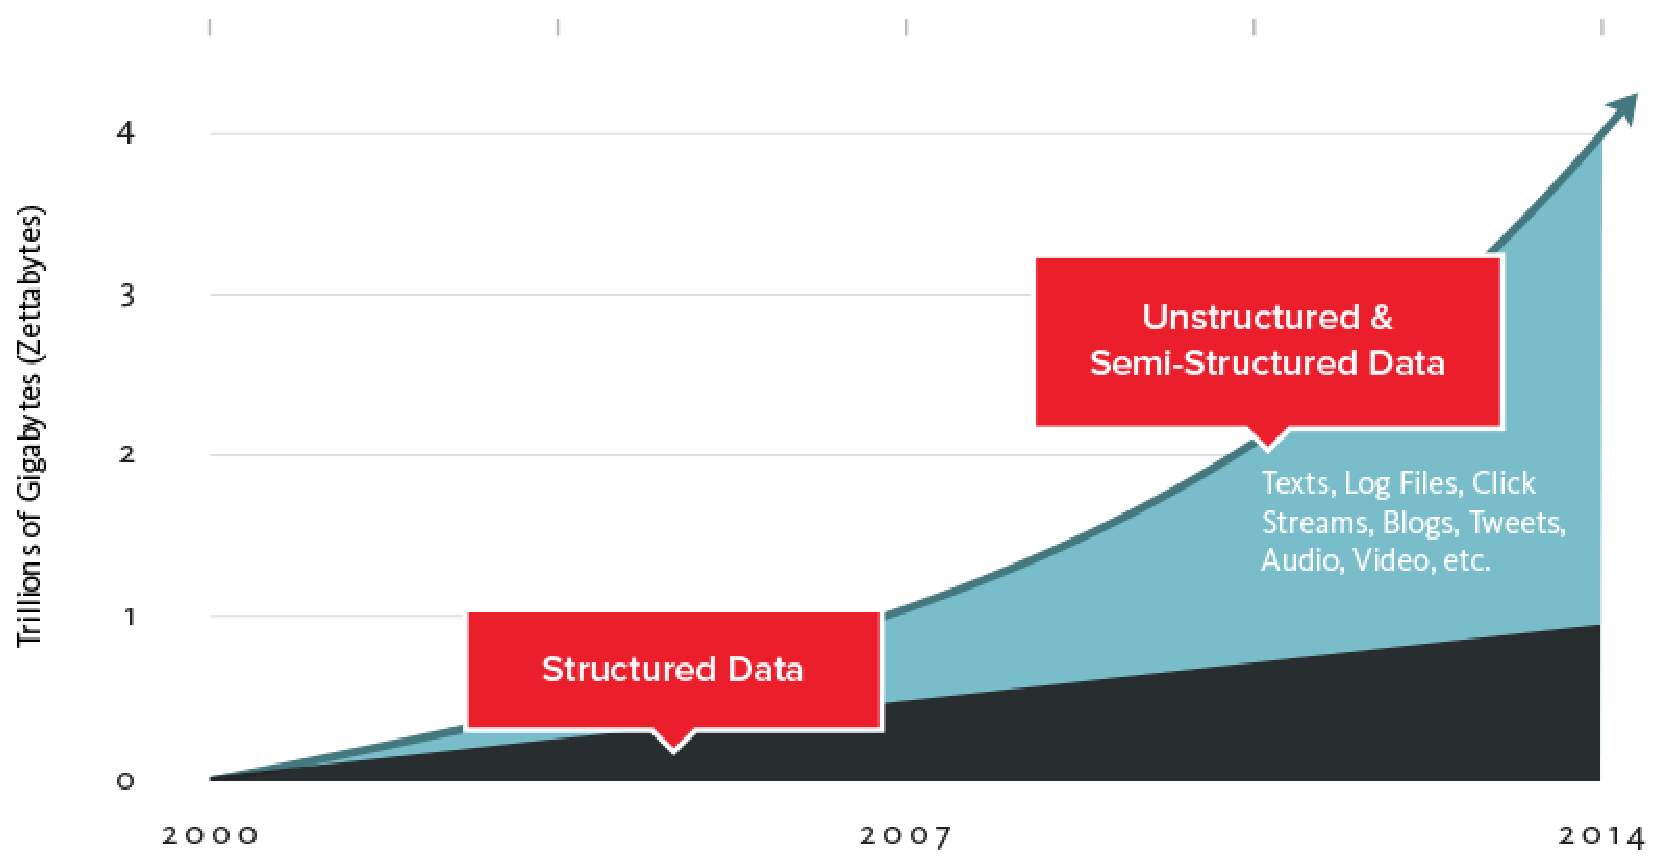
\includegraphics[width=10cm]{./img/why-nosql-2.eps}
		\caption{\tiny{Source: \url{http://www.couchbase.com/nosql-resources/what-is-no-sql}}}
	\end{figure}
\end{frame}

\begin{frame}
	\frametitle{How big are Big data?}
	\visible<2,3> {
		\begin{figure}
			\centering
			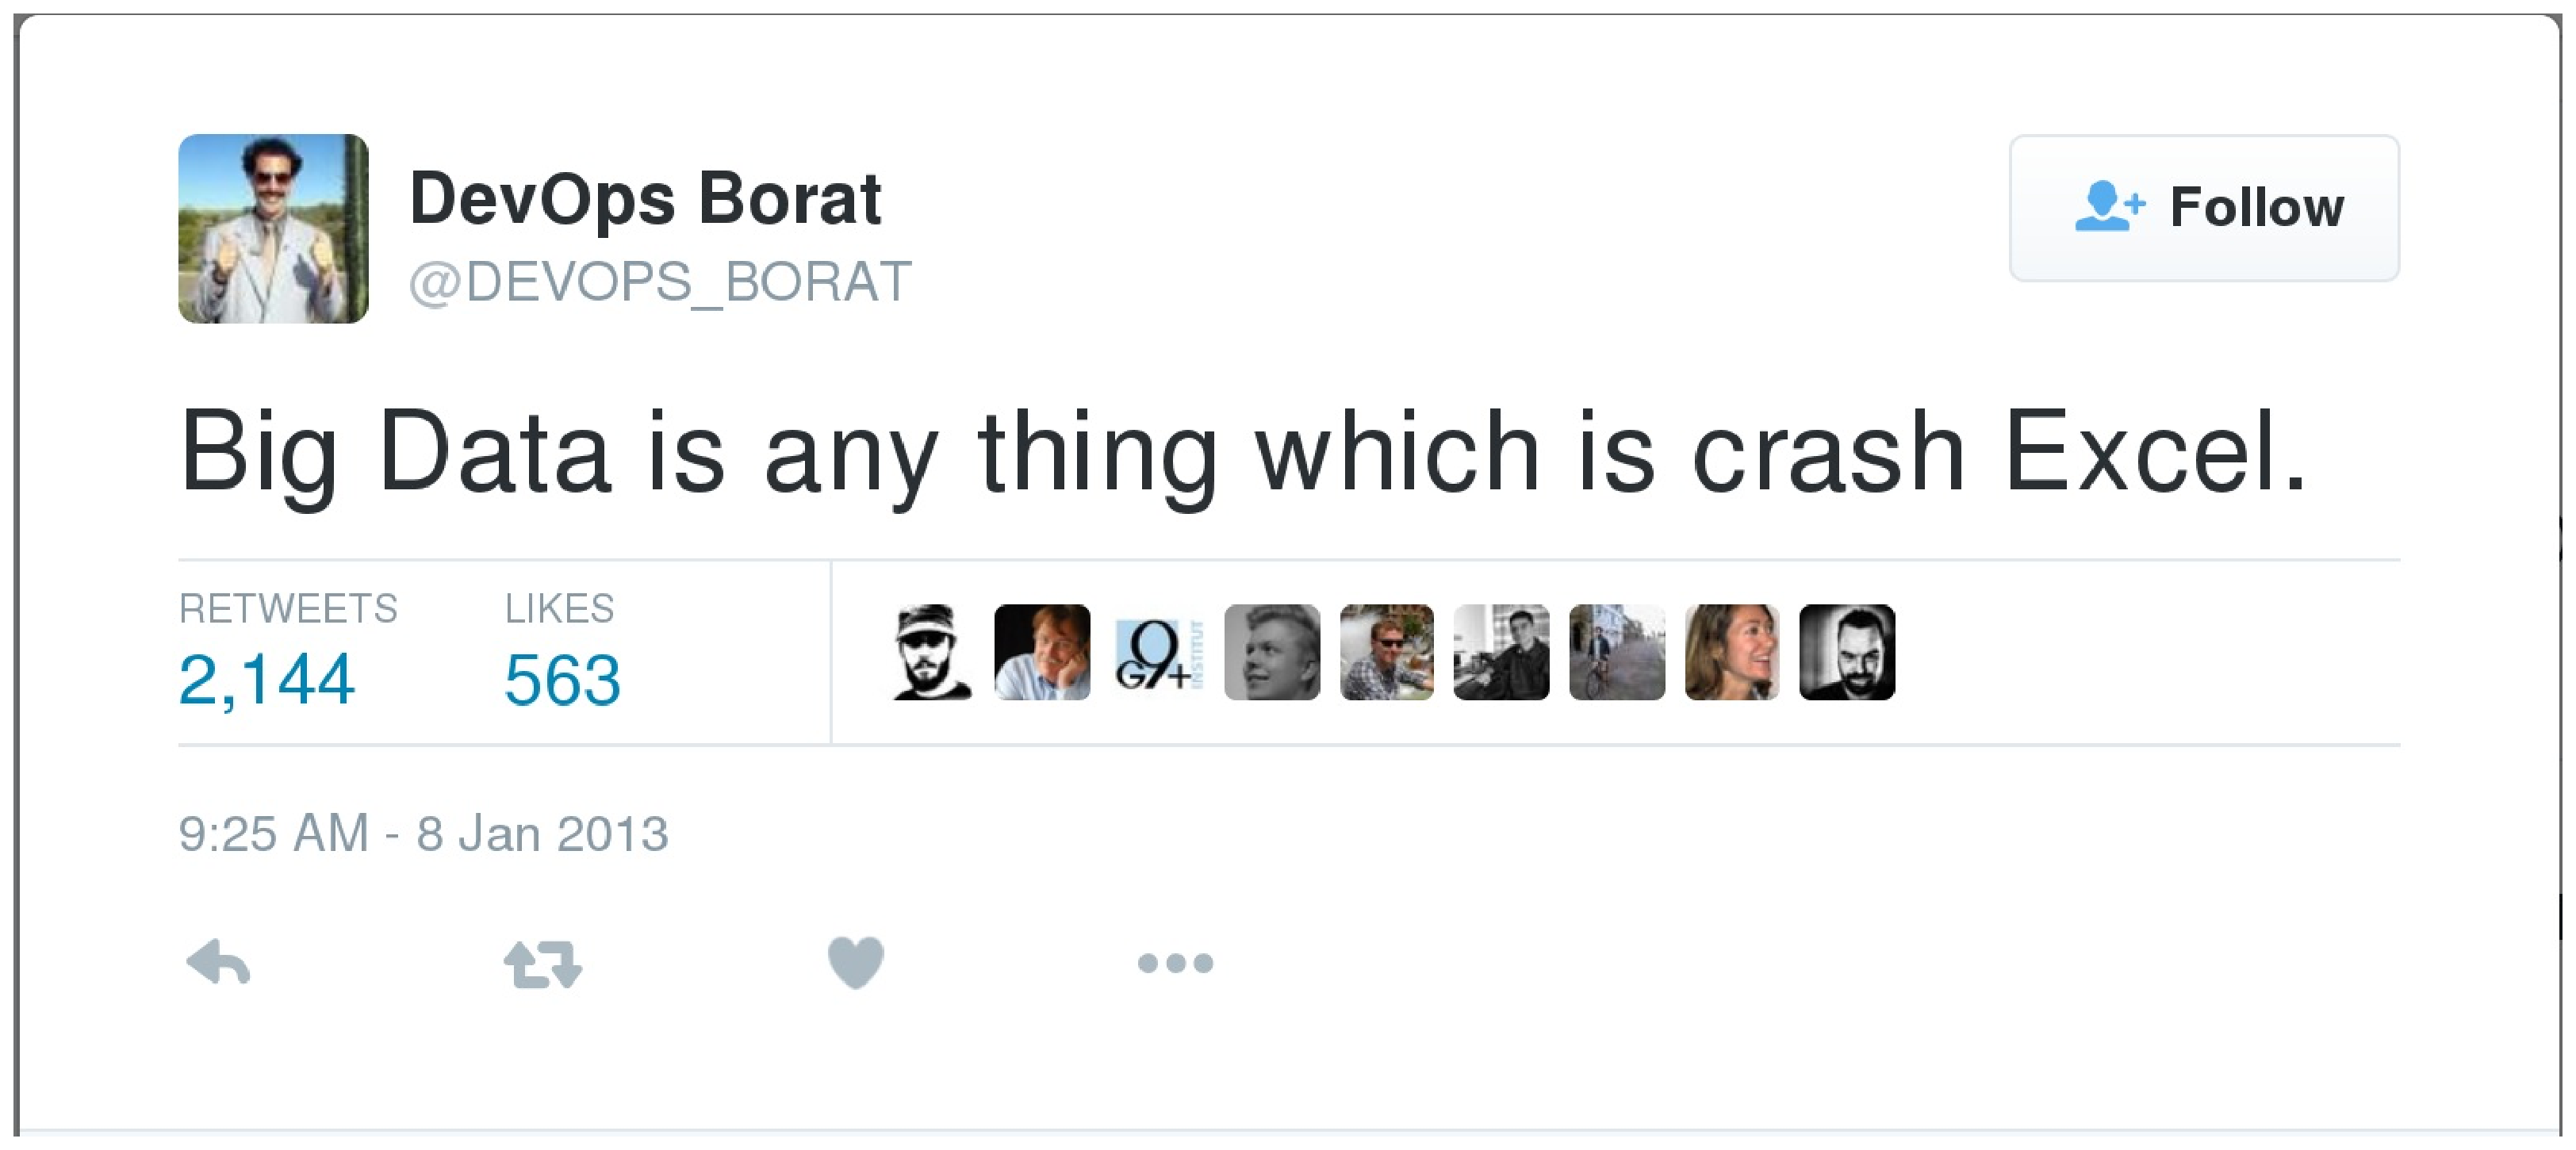
\includegraphics[width=8cm]{./img/borat_big_data.eps}
			\caption{\tiny{Source: \url{https://twitter.com/DEVOPS\_BORAT/status/288698056470315008}}}
		\end{figure}
	}
	\visible<3> {
		\begin{itemize}
			\item You can scale up, but sooner or later you'll probably have to scale out
			\item Need for highly scalable solution also because of cost effectiveness
		\end{itemize}
	}
\end{frame}

\begin{frame}
	\frametitle{Why NoSQL}
	\begin{itemize}
	 \item More flexible data mode
	 \item Better scalablity
	 \item Performance
	\end{itemize}
	\begin{figure}
		\centering
		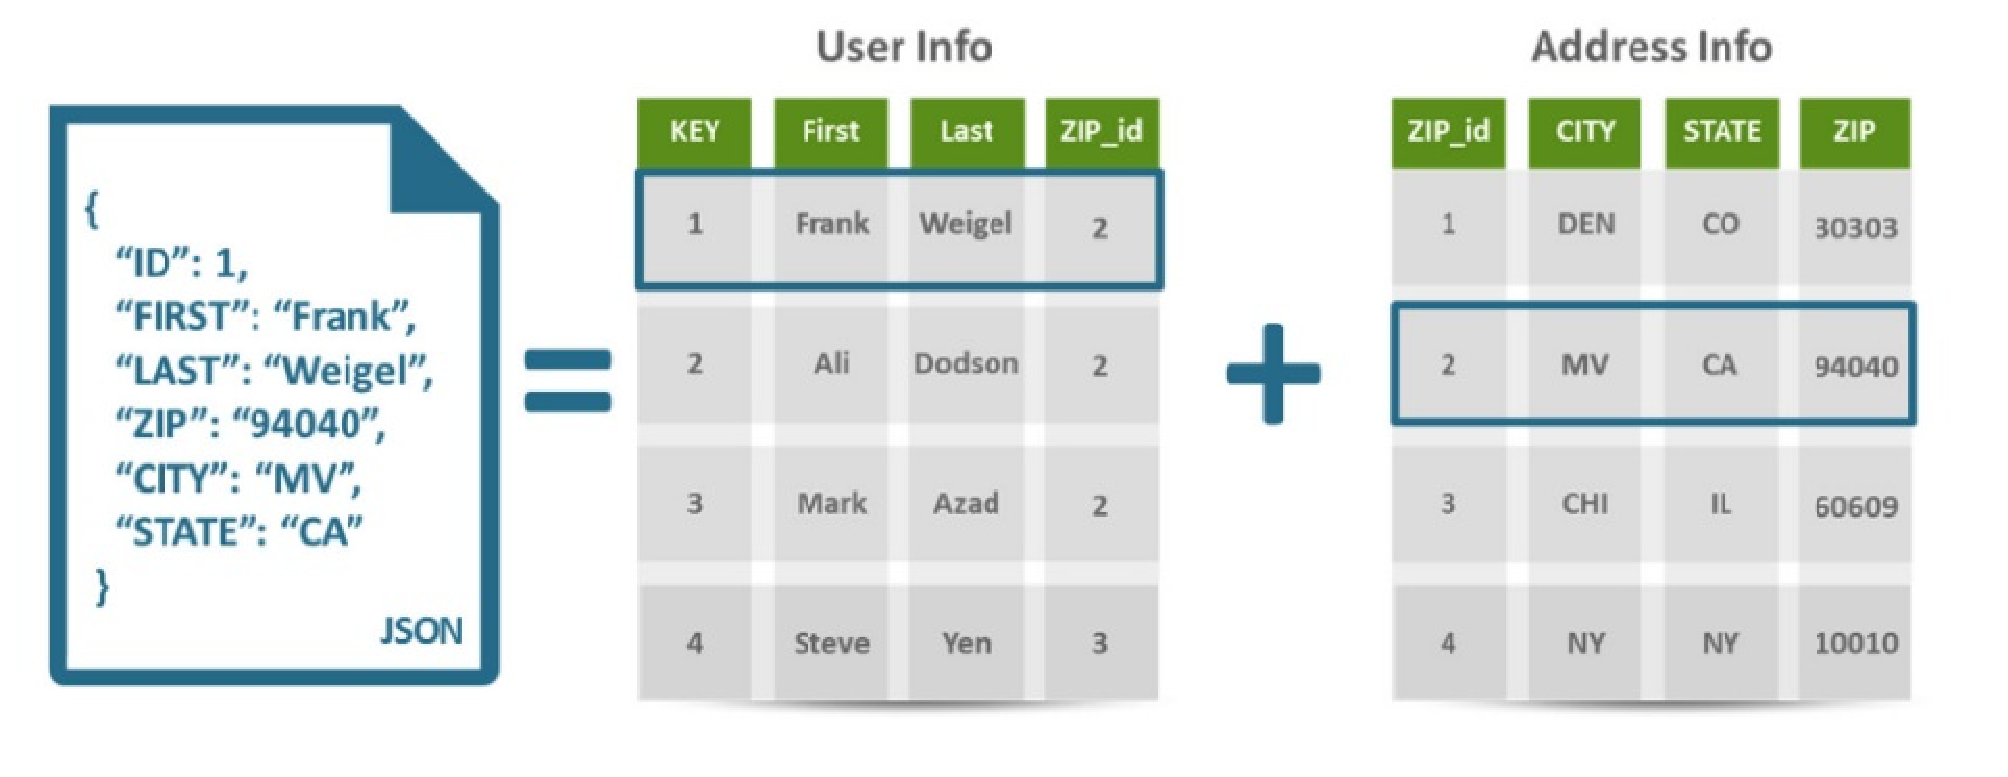
\includegraphics[width=10cm]{./img/json_vs_sql.eps}
		\caption{\tiny{Source: \url{www.couchbase.com/sites/default/files/uploads/all/whitepapers/NoSQL-Whitepaper.pdf}}}
	\end{figure}
\end{frame}


\begin{frame}
	\frametitle{Big data - challenges and approaches}
	\visible<1,2> {
		\begin{itemize}
			\item Analysis run on top of the huge amount of data
			\item Ability to store huge amount of unstructured data (often for performance reasons)
			\item Scalable solution
			\item Cloud architecture - everything is ephemeral
			\item But also ability  to talk to RDBMS or query structured data is often needed as well
		\end{itemize}
	}
	\visible<2> {
		\begin{figure}
			\centering
			
\includegraphics[width=10cm]{./img/borat_learn_nosql.eps}
			\caption{\tiny{Source: \url{https://twitter.com/devops_borat/status/141368065110708224}}}
		\end{figure}
	}
\end{frame}

\begin{frame}
	\centering
	\huge{\textbf{What's Infinispan}}
\end{frame}

\begin{frame}
	\frametitle{Infinispan}
	\begin{columns}
	\column{0.38\textwidth}
		\begin{figure}
			\centering
			
\includegraphics[width=3cm]{./img/infinispan.eps}
		\end{figure}
		\vspace{0.38cm}
		\color{blue}
			\url{https://infinispan.org}\\
			\vspace{0.1cm}
			\scriptsize{\url{https://github.com/infinispan}}\\
		\color{black}
		\scriptsize{(Apache License, v2.0)}
	\column{0.6\textwidth}
		\begin{itemize}
			\item In-memory data grid platform, written in Java
			\item Schema-less (optionally), No-SQL key-value data store
			\item Distributed cache - offers massive memory
			\item Elastic and scalable - can run on hundreds of nodes
			\item Highly available - no SPOF, resilient to node failures
			\item Concurrent (MVCC)
			\item Transactional
			\item Queryable
			\item Processing for streaming data
		\end{itemize}
	\end{columns}
\end{frame}

\begin{frame}
	\frametitle{Why in-memory}
	\begin{itemize}
	 \item Lots of data is needed in real-time (BigData $\rightarrow$ FastData)
	 \item Some tasks can be completed much faster when data are kept in memory
	 \item Keeping data in memory during processing of whole application stack, not only during processing in one application in the stack
	 \item With data replication you can keep your data only in memory (no need to store them in persistent storage)
	\end{itemize}
\end{frame}

\begin{frame}
	\frametitle{Why caching}
	\begin{figure}
		\centering
		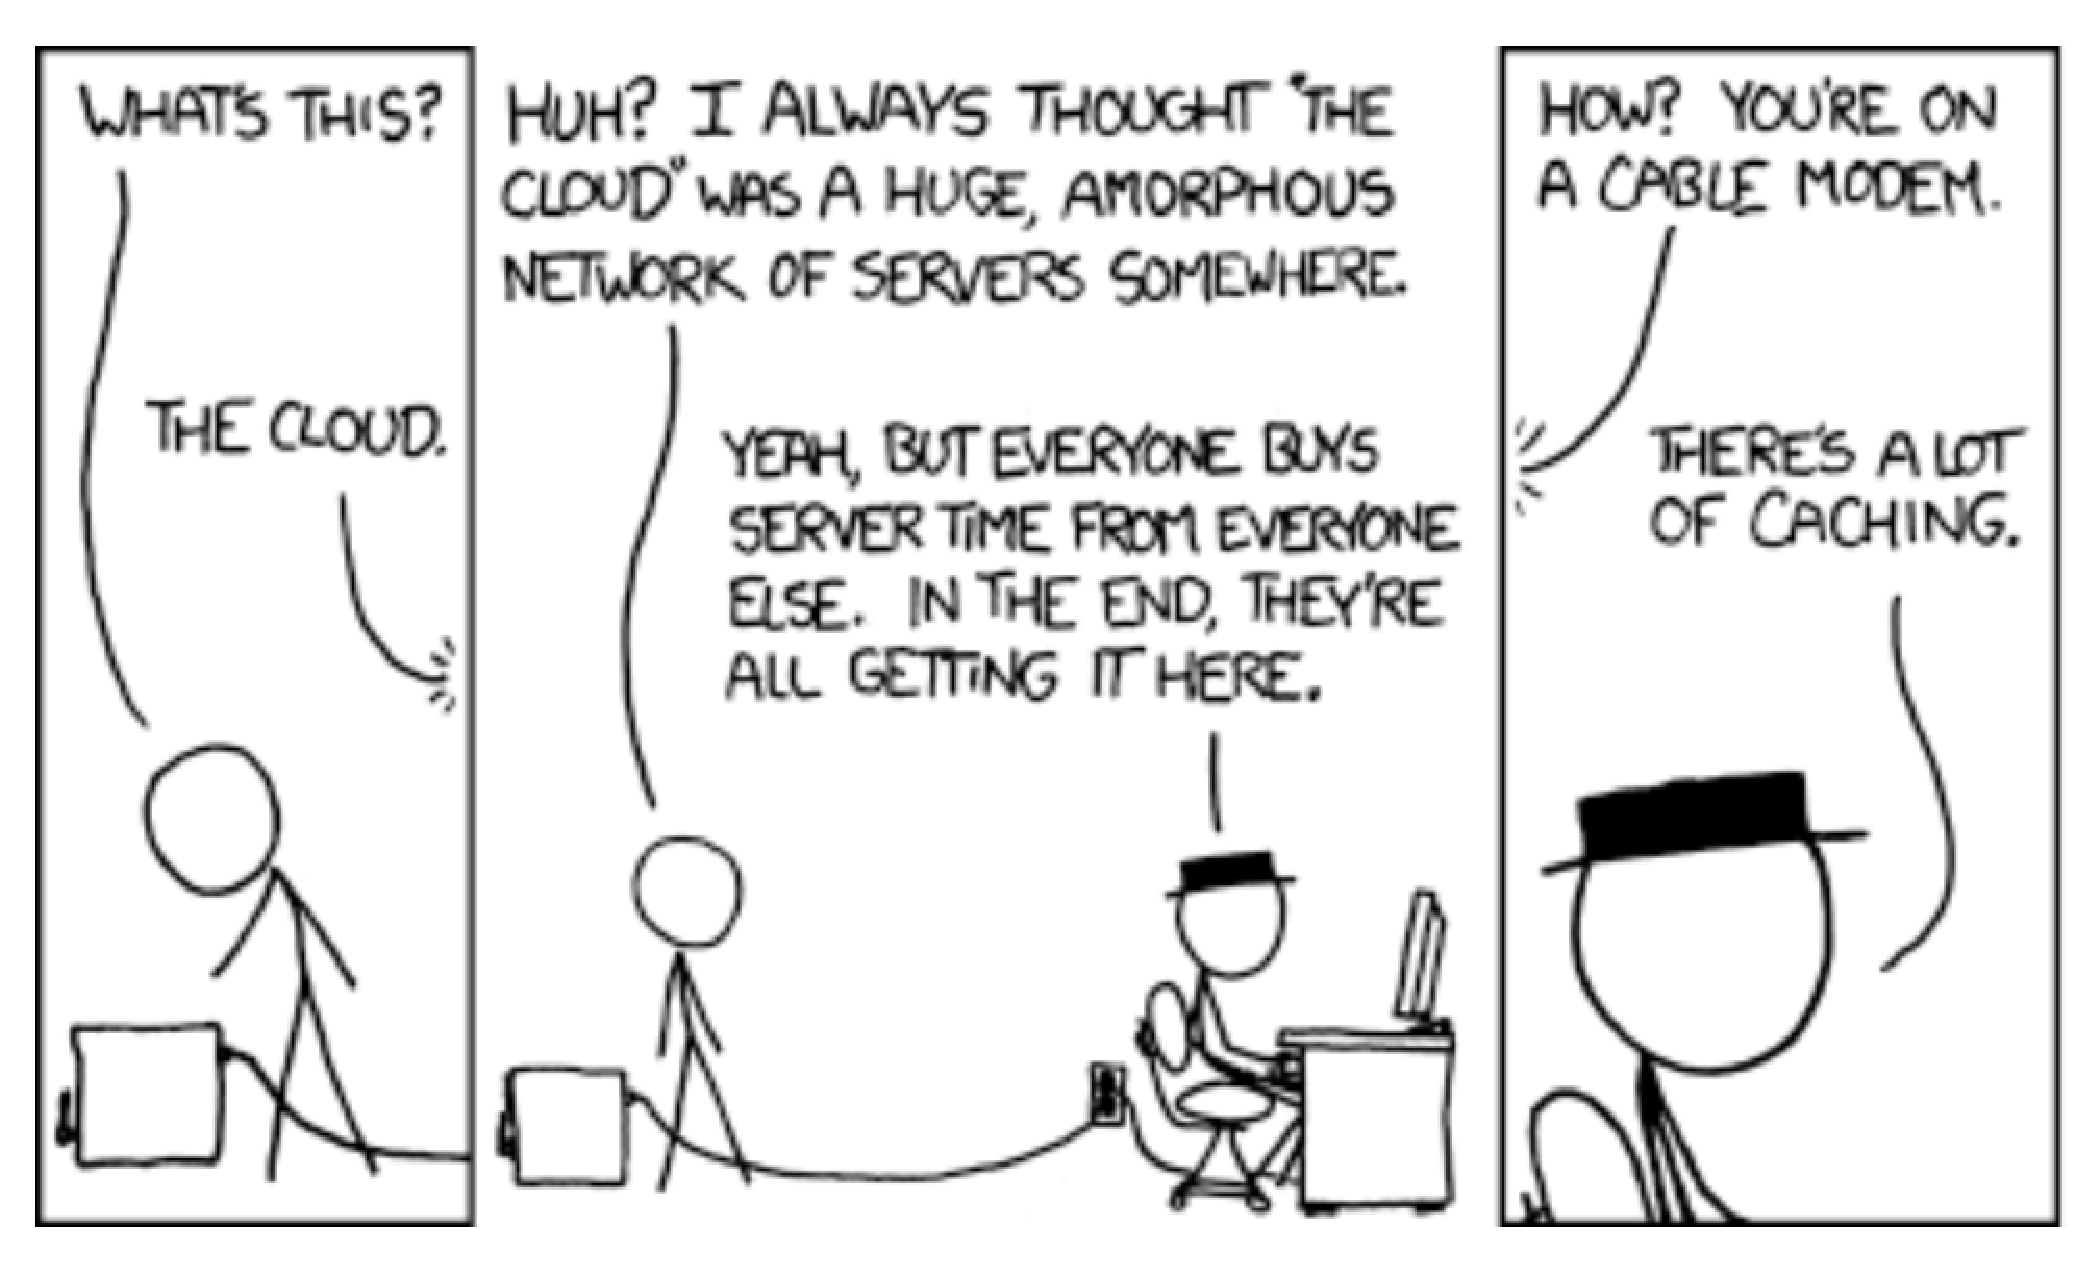
\includegraphics[width=12cm]{./img/xkcd_908.eps}
		\caption{\tiny{Source: Part of \href{http://xkcd.com/908/}{xkcd \#908}}}
	\end{figure}
\end{frame}

\begin{frame}[fragile]
	\frametitle{Infinispan cache}
	\begin{itemize}
		\item Infinispan takes care about all that hard stuf.
		\item From user perspective Infinispan cache is \textbf{just a map!}
	\end{itemize}
	\vspace{0.3cm}
	\begin{lstlisting}[style=Java]
		DefaultCacheManager cacheManager = new DefaultCacheManager("my_ispn_config.xml");
		Cache<String, String> cache = cacheManager.getCache("myCache");
		cache.put("key", "value");
		String value = cache.get("key");
	\end{lstlisting}
\end{frame}


\begin{frame}
  \frametitle{Infinispan modes}
	\begin{columns}
	\column{0.5\textwidth}
		\begin{itemize}
			\item Embedded (library, in-VM)
		\end{itemize}
		\begin{figure}
			%\centering
			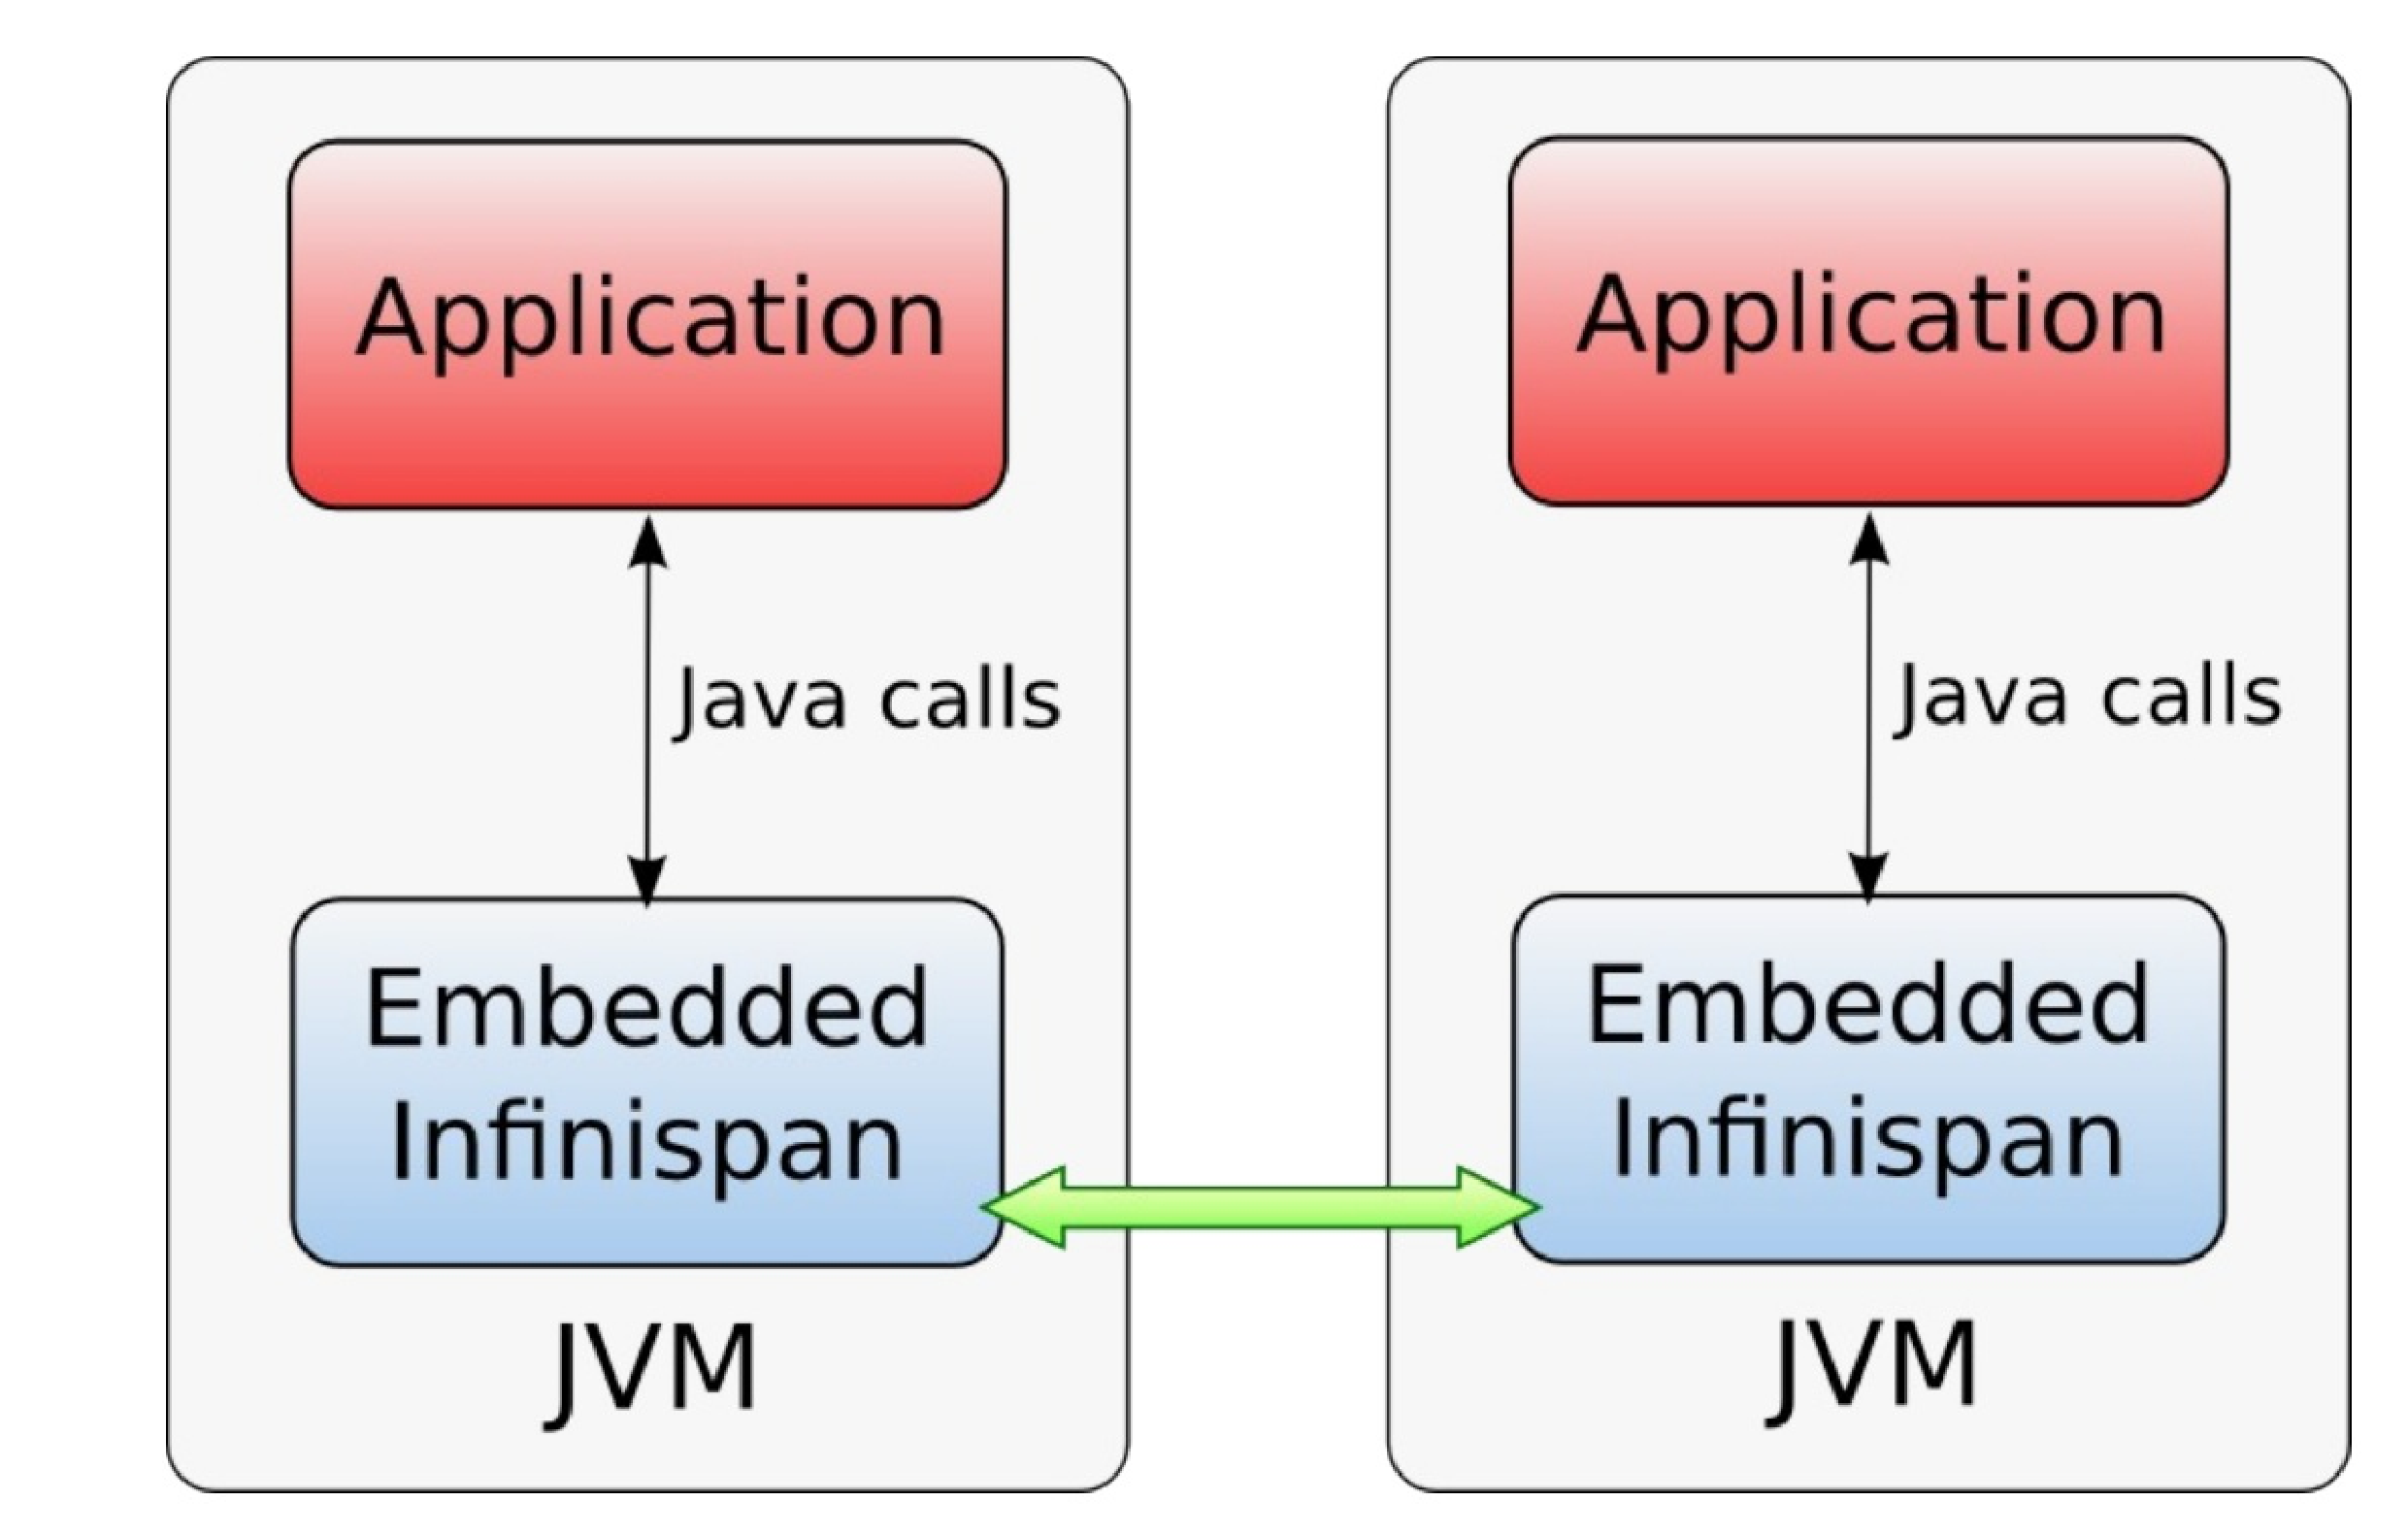
\includegraphics[width=5cm]{./img/ispn-emb.eps}
		\end{figure}
	\column{0.5\textwidth}
		\begin{itemize}
			\item Client-server (remote)
		\end{itemize}
		\begin{figure}
			%\centering
			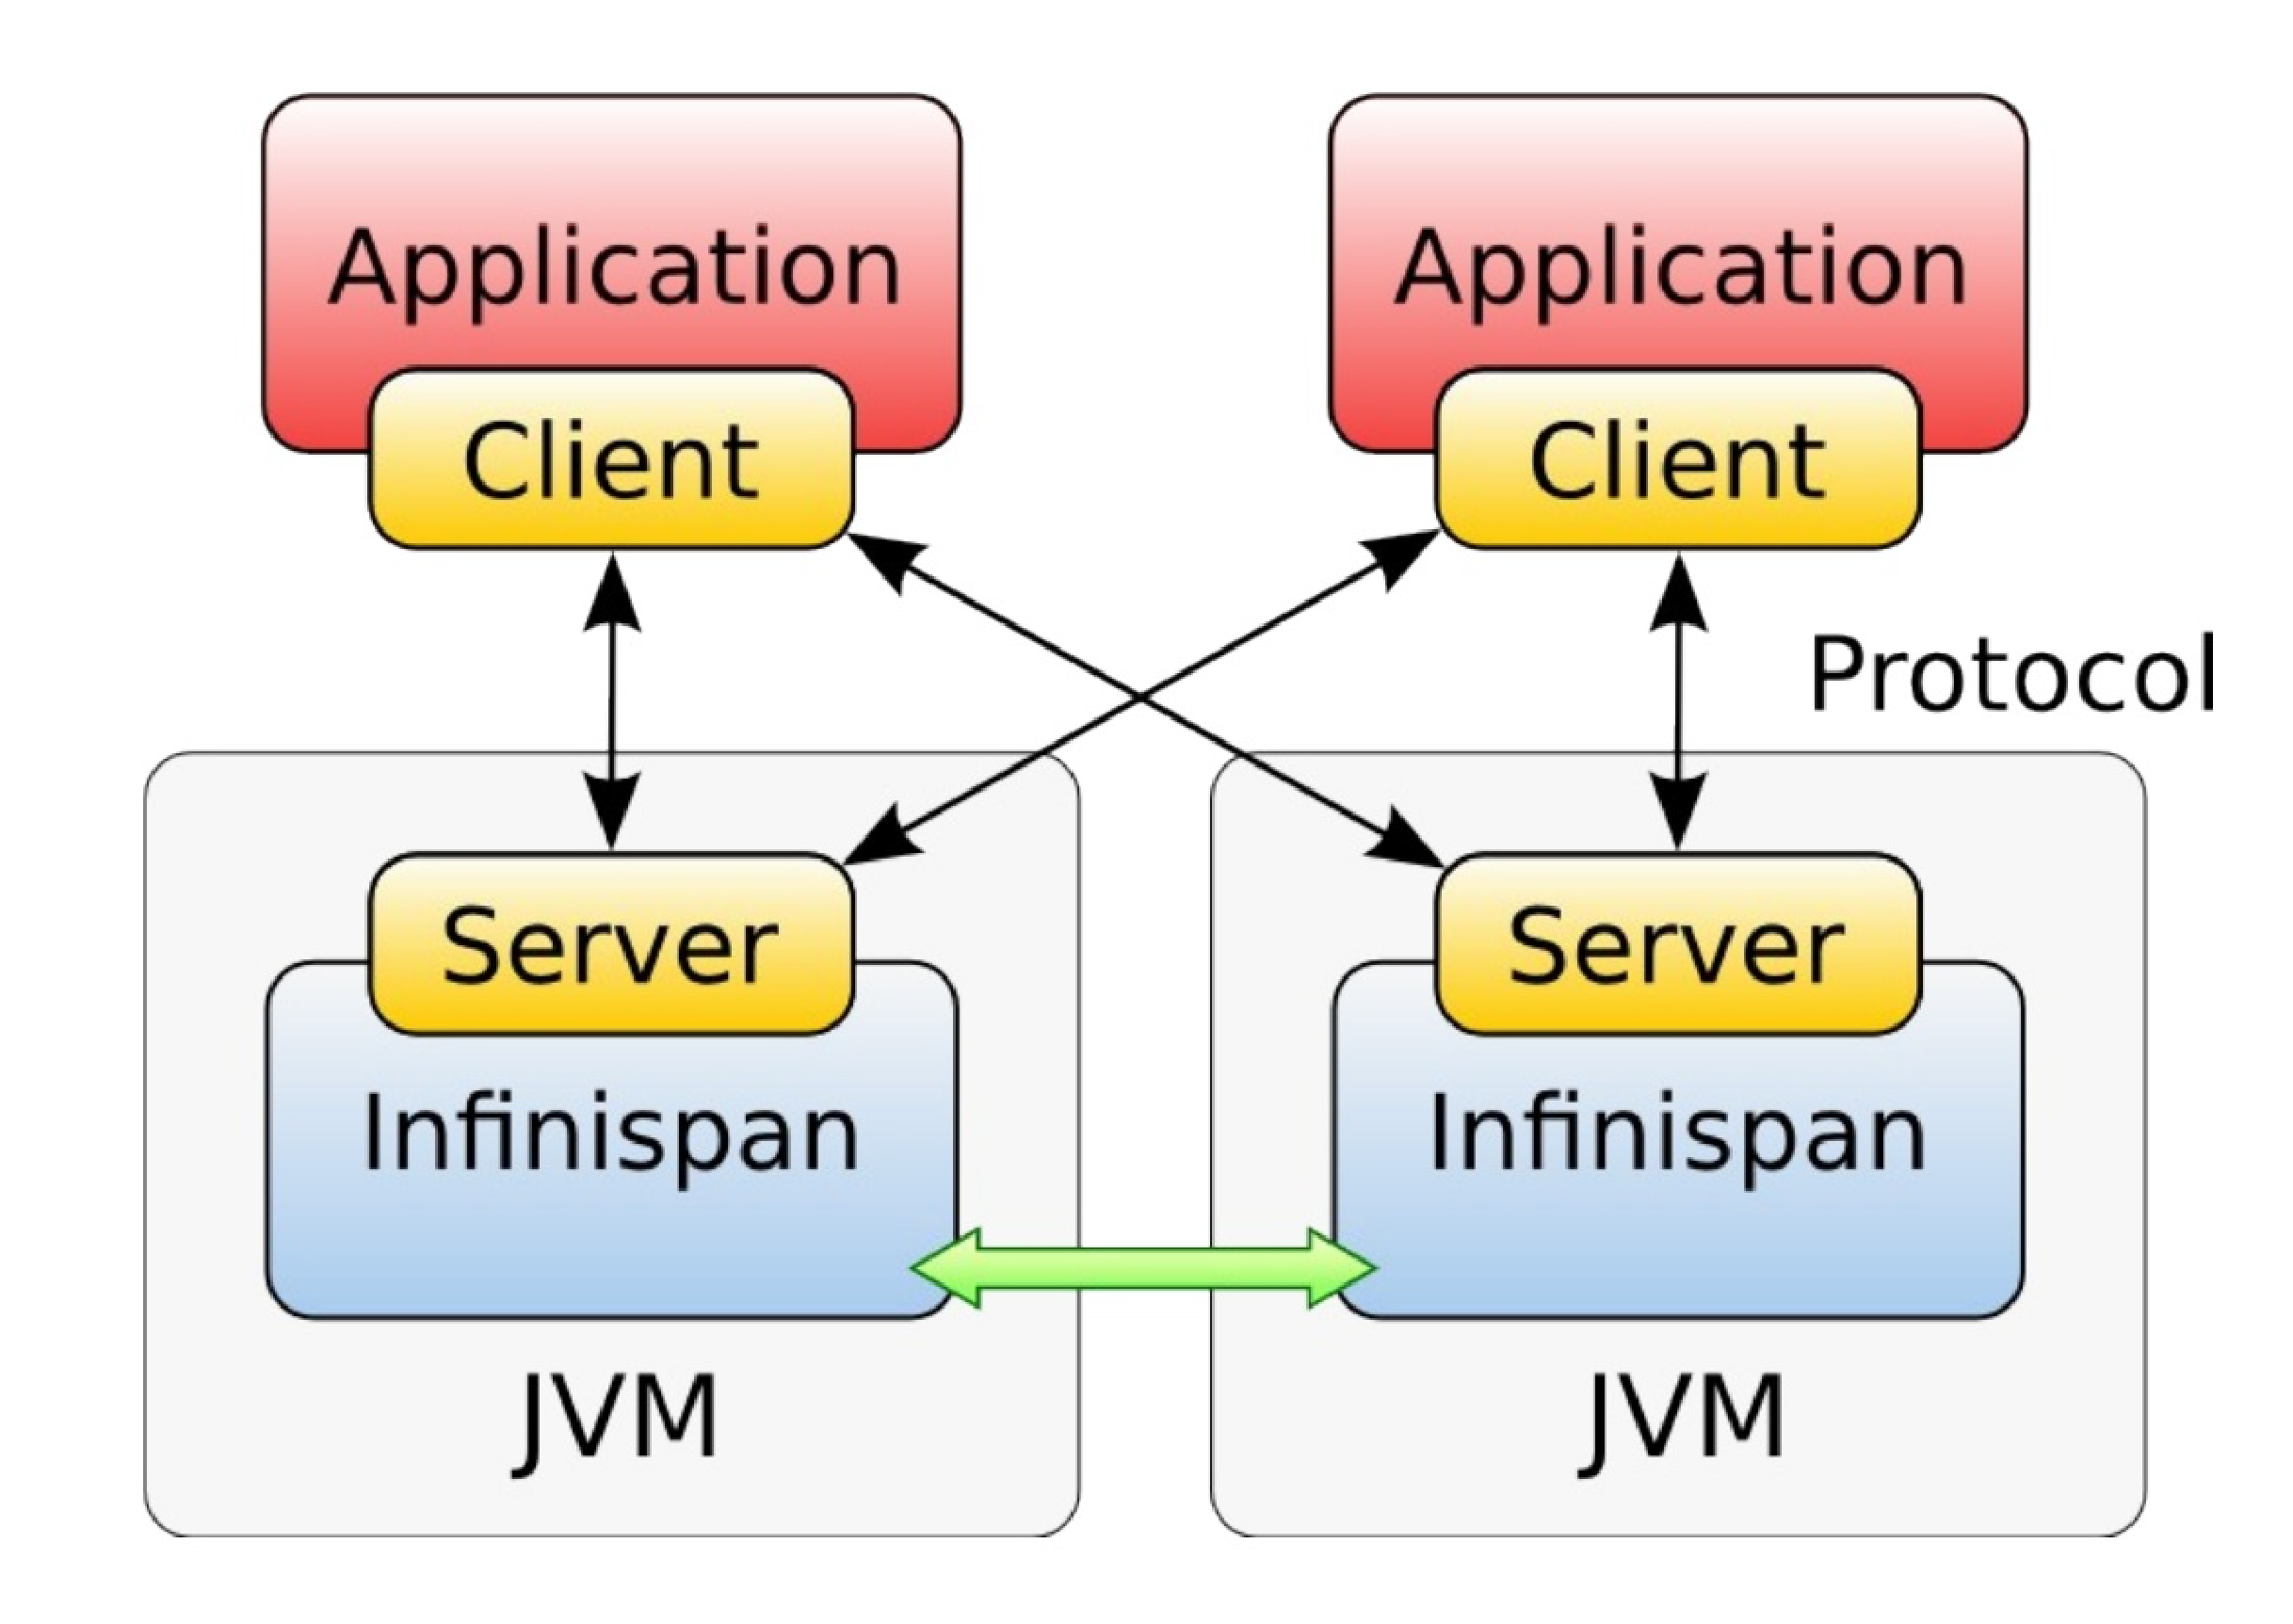
\includegraphics[width=5cm]{./img/ispn-cs.eps}
		\end{figure}
	\end{columns}
\end{frame}

\begin{frame}
	\frametitle{Clustering modes}
	Under the hood leverages JGroups project for clustering.
	\begin{columns}
	\column{0.5\textwidth}
		\begin{itemize}
			\item Local - no clustering
			\vspace{3cm}
			\item Replicated
			\begin{figure}
				%\centering
				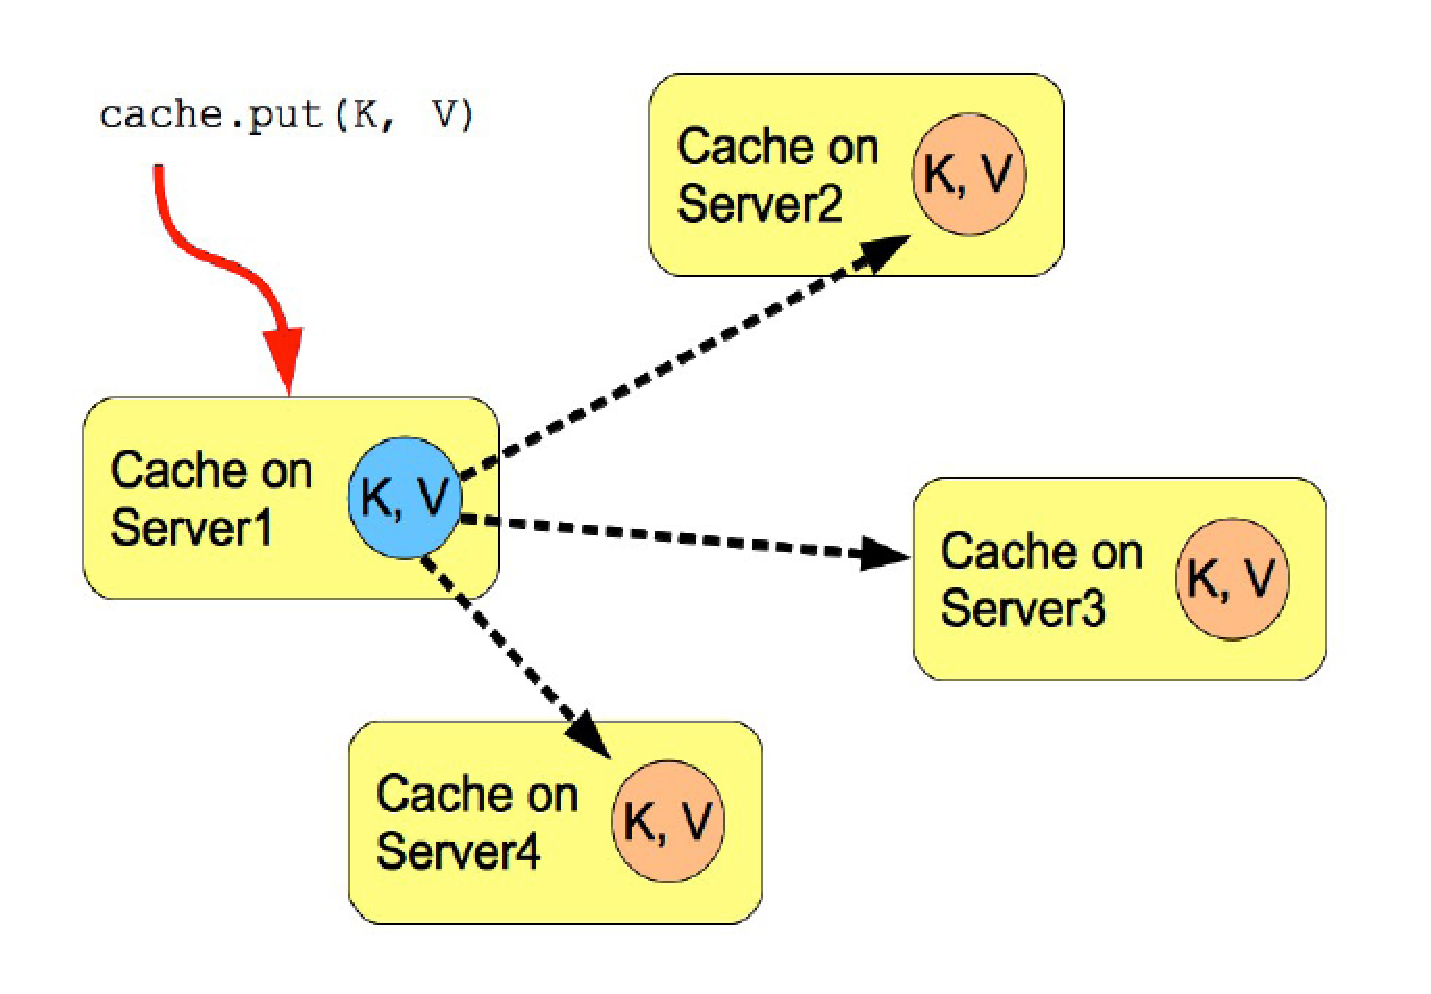
\includegraphics[width=4cm]{./img/ispn-repl.eps}
			\end{figure}
		\end{itemize}
	\column{0.5\textwidth}
		\begin{itemize}
			\item Invalidation
			\begin{figure}
				%\centering
				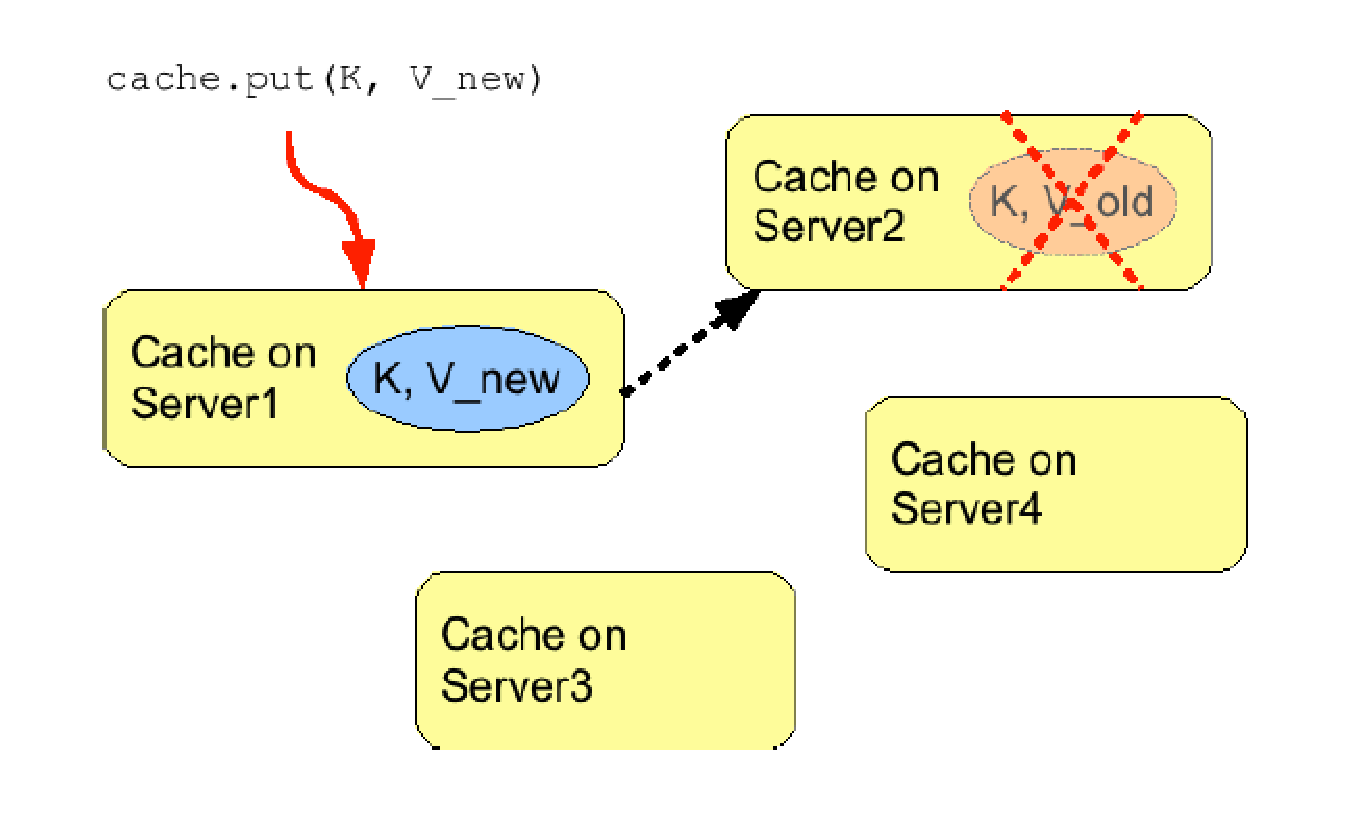
\includegraphics[width=4cm]{./img/ispn-inval.eps}
			\end{figure}
			\item Distributed
			\begin{figure}
				%\centering
				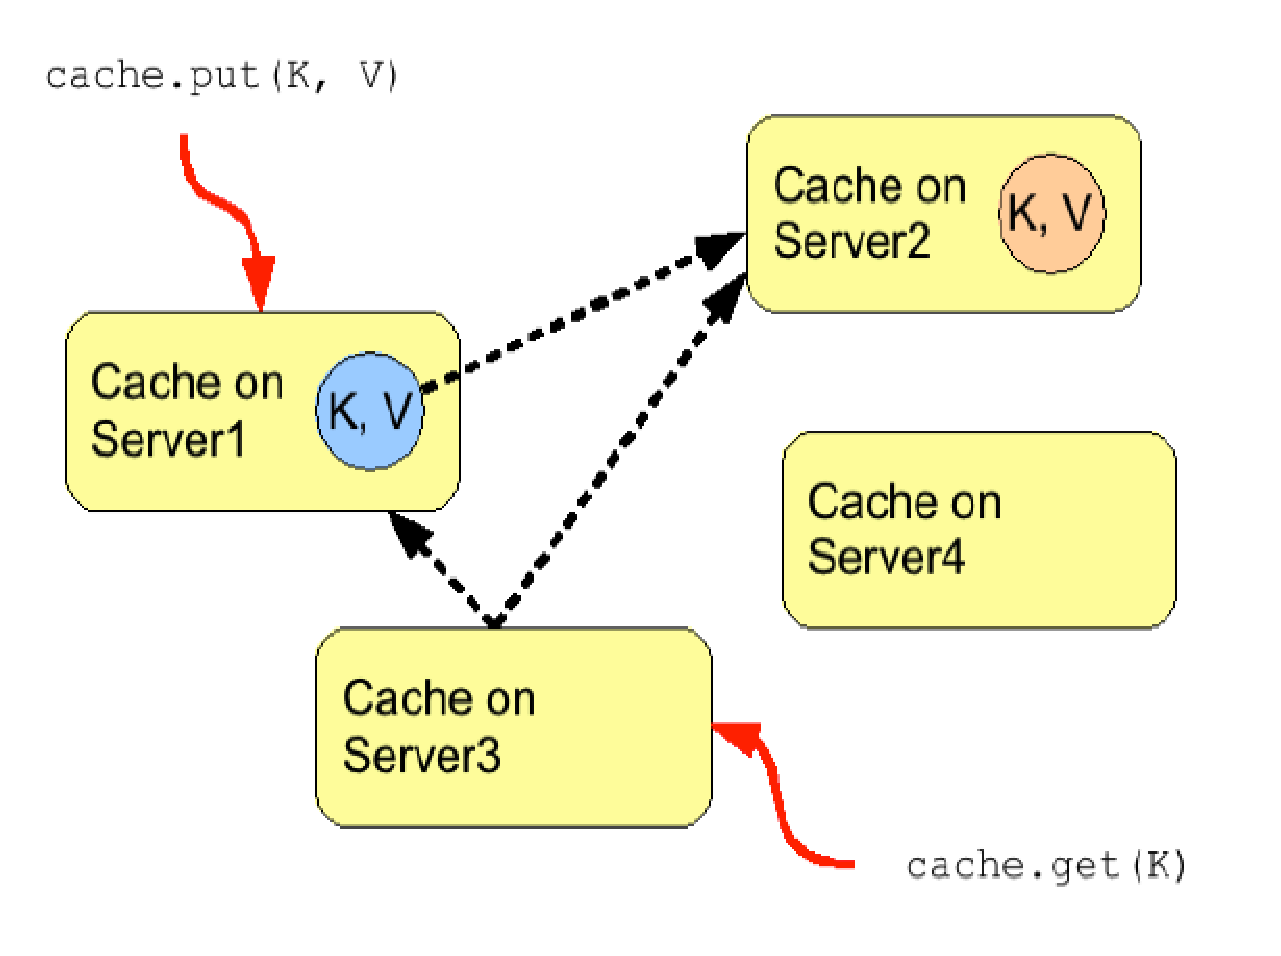
\includegraphics[width=4cm]{./img/ispn-dist.eps}
			\end{figure}
		\end{itemize}
	\end{columns}
\end{frame}


\begin{frame}
	\frametitle{Remote protocols}
	\begin{columns}
	\column{0.5\textwidth}
		\begin{itemize}
			\item Hot Rod
				\begin{itemize}
					\item hashing and topology aware
					\item failover during topology changes
					\item smart request routing
				\end{itemize}
			\item Memcached
			\item REST
		\end{itemize}
	\column{0.5\textwidth}
		\begin{figure}
			%\centering
			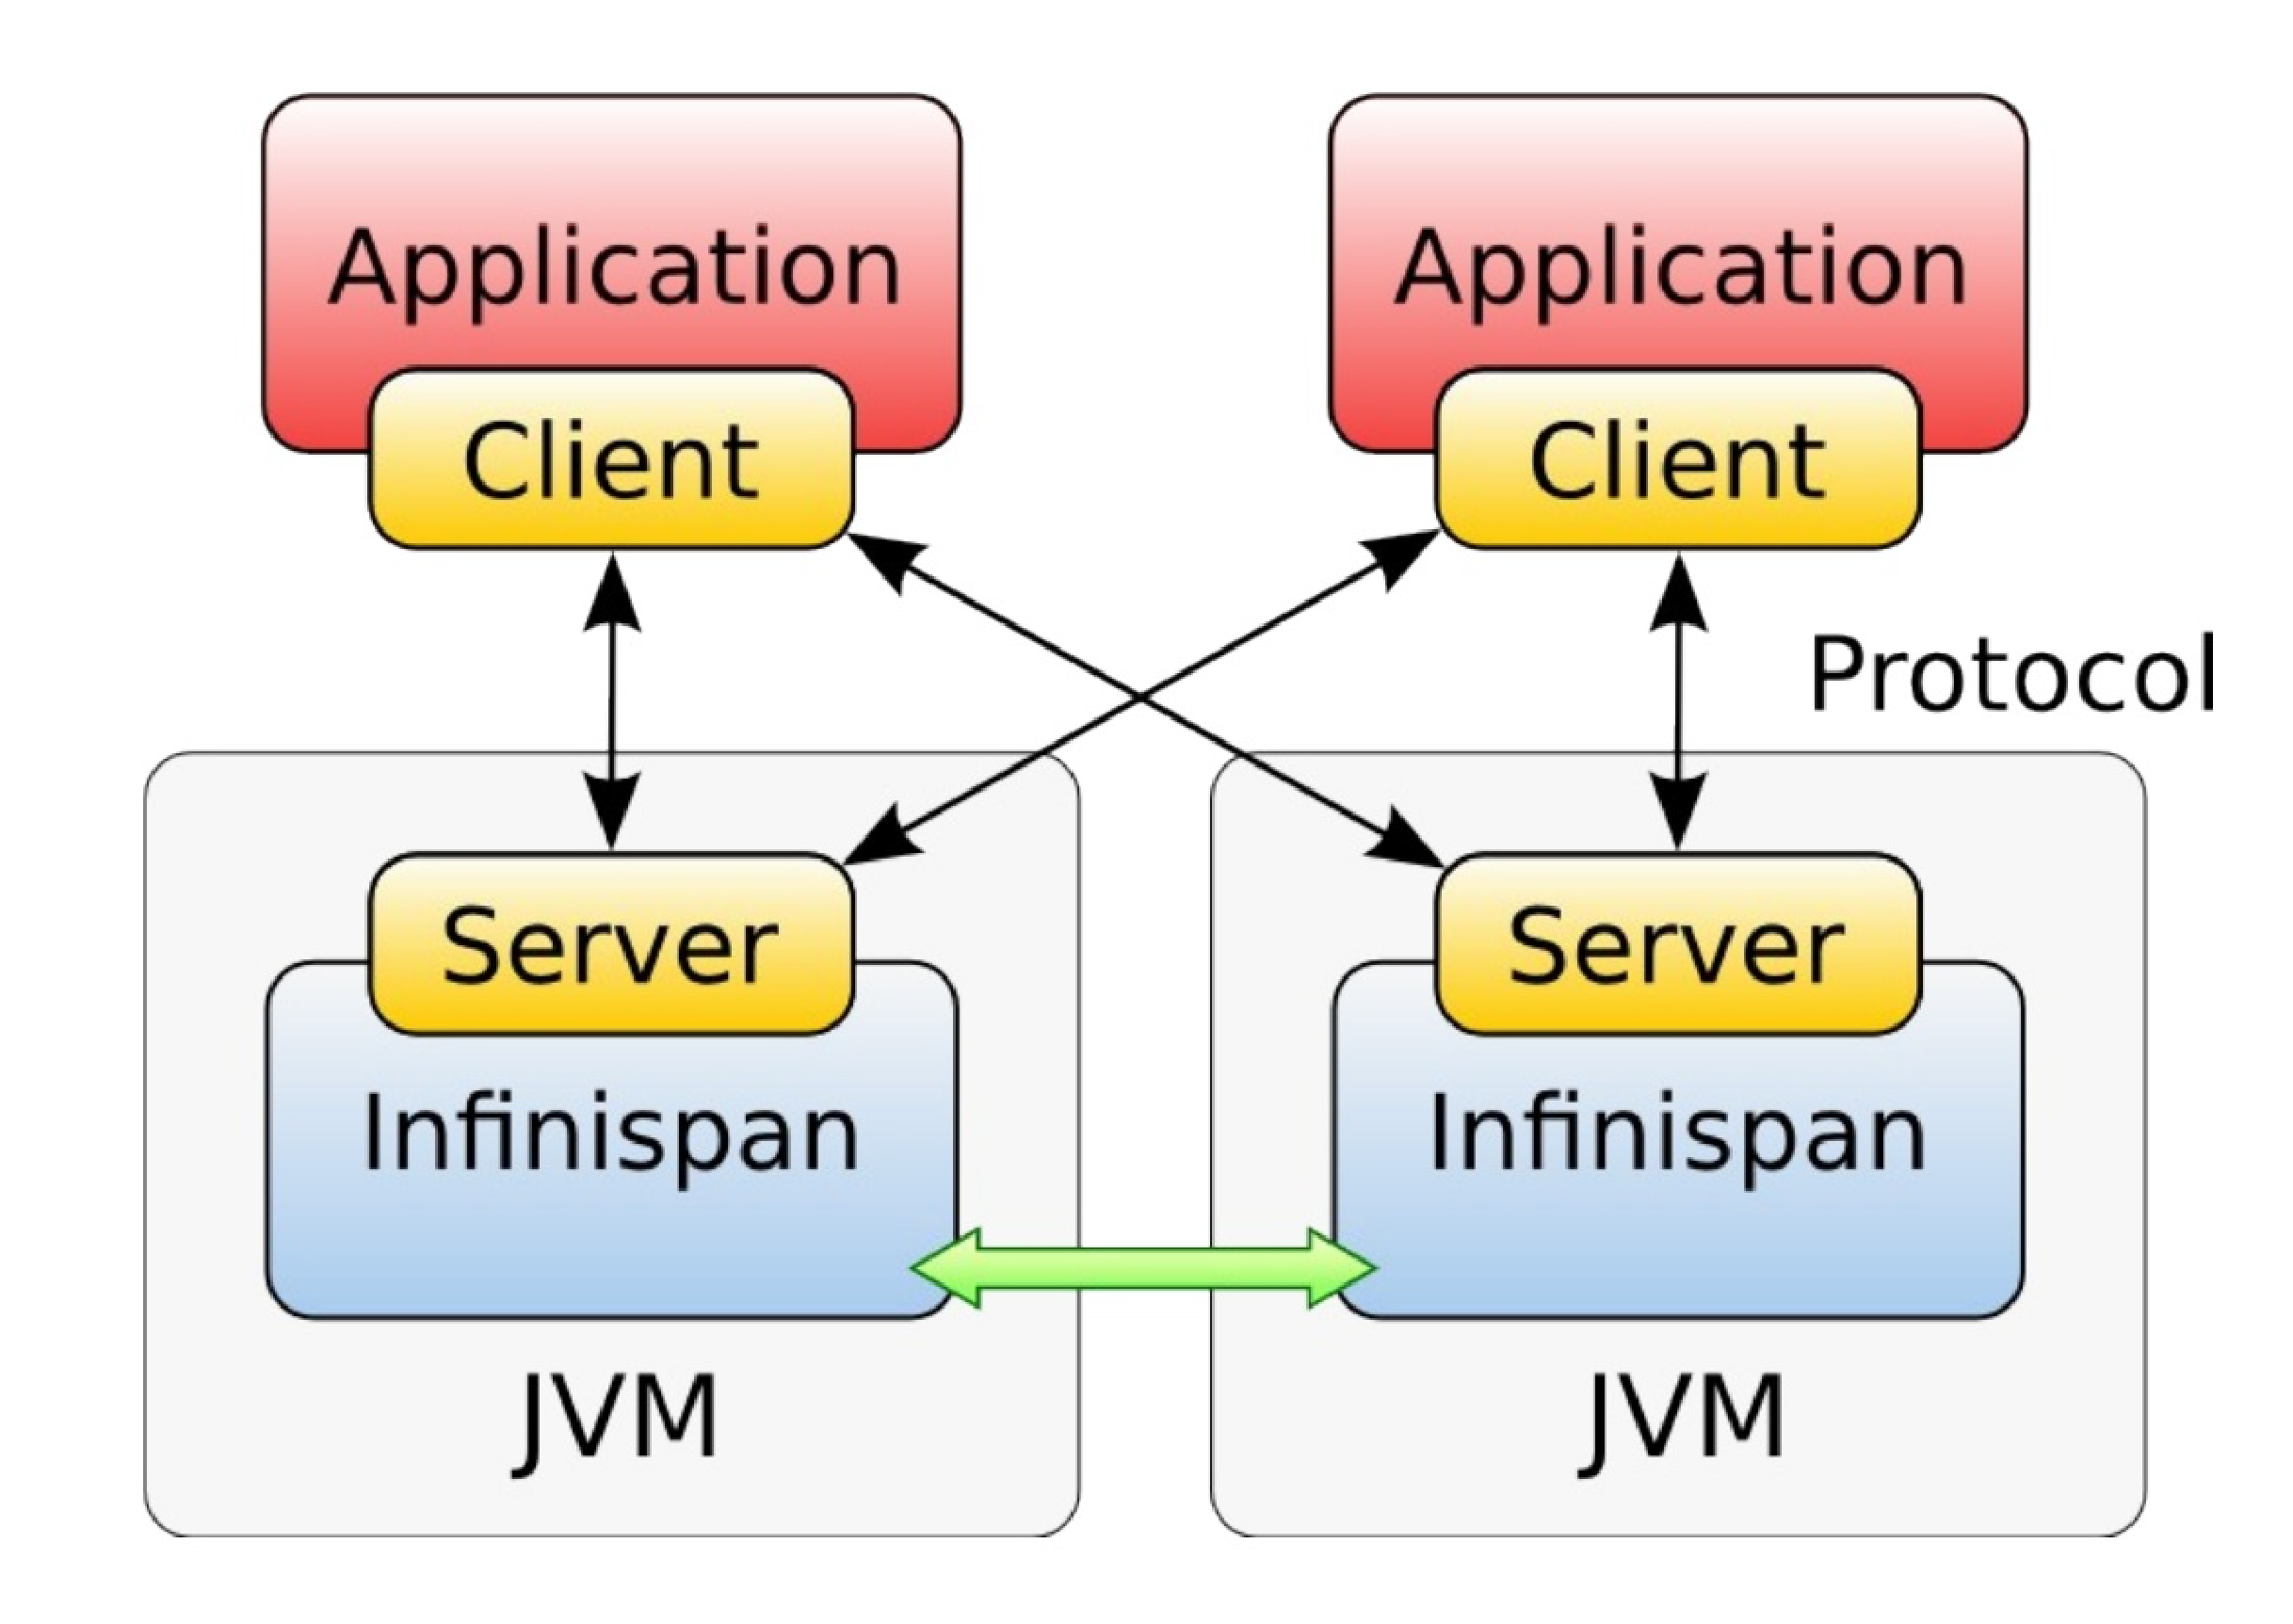
\includegraphics[width=5cm]{./img/ispn-cs.eps}
		\end{figure}
	\end{columns}
\end{frame}

\begin{frame}
  \frametitle{Hot Rod clients}
	Compatible with Java and non-Java platforms. Based on Protocol Buffers - Google's data interchange format.\\
	\vspace{0.5cm}
	Clients for
	\begin{itemize}
		\item Java
		\item C\#
		\item C++
		\item Python
		\item Ruby
	\end{itemize}
	Python and Ruby clients have only basic functionality.
\end{frame}

\begin{frame}
	\frametitle{Cache stores}
	A way how to store cache content in some external (persistent) storage.\\
	Two modes:
	\begin{itemize}
	 \item Synchronous (write-through)
	 \item Asynchronous (write-behind)
	\end{itemize}
	Cache stores:
	\begin{itemize}
		\item Single file store and soft-index file store
		\item JDBC and JPA cache stores
		\item LevelDB cache store
		\item Cloud cache store
		\item Remote store
		\item \dots and others
  \end{itemize}
	Also possible to define custom cache store.
\end{frame}

\begin{frame}
	\frametitle{Transactions}
	\begin{itemize}
	 \item JTA-compliant transactions
	 \item Ensures consistency of data
	 \item Optimistic and pessimistic locking available
	 \item Read committed and repeatable read isolation levels
	 \item Deadlock detection and recovery
	 \item Data versioning
% 		\begin{itemize}
% 			\item Simple versioning
% 			\item Partition-aware versioning (vector locks)
% 			\item External versioning - used e.g. with Hibernate, where locks are provided by database
% 		\end{itemize}
	\end{itemize}
\end{frame}

\begin{frame}
	\frametitle{Querying}
	\begin{itemize}
		\item Needs some data schema (protobuf file or annotations)
		\item Search for data using data attributes instead of keys
		item Featured attributes include keyword, range, fuzzy, wildcard, and phrase queries.
		\item Combine queries and aggregation functions (but doesn't support joins)
		\item Sort, filter, and paginate query results
		\item Support for index or non-indexed queries
% 		\item Allows for indexing of entries as they are stored
% 		\item Indexing
		\item Lucene query API or fluent DSL API
	\end{itemize}
\end{frame}

\begin{frame}
	\frametitle{Security}
	\begin{itemize}
	 \item Role based access control
	 \item User authentication
	 \item Node authentication and authorization
	 \item Encryption of communication
	 \item Audit logging
	 \item Integration with LDAP and/or Kerberos server (includes Active Directory)
	\end{itemize}
\end{frame}


\begin{frame}
  \frametitle{Some other features - brief and selective list}
  \begin{itemize}
		\item Data eviction
		\item Full JSR-107 support (Java Temporary Caching API)
		\item CDI support
		\item Remote events
		\item Client near cache
		\item Rolling upgrades
		\item Cross data center replication (also Hot Rod clients support failover to another data center)
		\item Command line interface
		\item Map-reduce framework and distributed executors
  \end{itemize}
\end{frame}


\begin{frame}
	\frametitle{Recently implemented features: Infinispan 8}
	\begin{figure}
		\centering
		
\includegraphics[width=5cm]{./img/infinispan8.eps}
	\end{figure}
  \begin{itemize}
    \item Functional API
		\item Distributed streaming
		\item Continuous querying, grouping and aggregation
		\item New management console
		\item Integration with Apache Spark and Hadoop
		\item \dots and more
  \end{itemize}
\end{frame}

\begin{frame}
	\frametitle{Integration with other frameworks}
	\begin{itemize}
		\item Hibernate
		\begin{itemize}
			\item 2-nd level cache
		\end{itemize}
		\item Lucene directory
		\begin{itemize}
		 \item In-memory Lucene index 
		\end{itemize}
		\item Apache Camel
		\begin{itemize}
		 \item Infinispan component for Camel
		\end{itemize}
		\item Hadoop
		\begin{itemize}
			\item In-memory data source for Hadoop cluster
		\end{itemize}
		\item Apache Spark
		\begin{itemize}
			\item Data source for Spark map-reduce jobs
		\end{itemize}
	\end{itemize}
\end{frame}

\begin{frame}
	\frametitle{Some projects using Infinispan}
	\begin{columns}
	\column{0.2\textwidth}
	\column{0.85\textwidth}
		\begin{itemize}
			\item WildFly
				\hspace{10cm}
				\begin{figure}
					\vspace{-1cm}
					
\includegraphics[height=0.75cm]{./img/wildfly.eps}
				\end{figure}
			\item Hibernate
				\hspace{10cm}
				\begin{figure}
					\vspace{-1cm}
					
\includegraphics[height=0.75cm]{./img/hibernate.eps}
				\end{figure}
			\item Apache Camel
				\hspace{10cm}
				\begin{figure}
					\vspace{-1cm}
					
\includegraphics[height=0.75cm]{./img/apache-camel.eps}
				\end{figure}
			\item Apache Marmotta
				\hspace{10cm}
				\begin{figure}
					\vspace{-1cm}
					
\includegraphics[height=0.75cm]{./img/marmotta.eps}
				\end{figure}
			\item CapeDwarf
				\hspace{10cm}
				\begin{figure}
					\vspace{-1cm}
					
\includegraphics[height=0.75cm]{./img/capedwarf.eps}
				\end{figure}
			\item Immutant
				\hspace{10cm}
				\begin{figure}
					\vspace{-1cm}
					
\includegraphics[height=0.75cm]{./img/immutant.eps}
				\end{figure}
			\item apiman
				\hspace{10cm}
				\begin{figure}
					\vspace{-1cm}
					
\includegraphics[height=0.5cm]{./img/apiman.eps}
				\end{figure}
			\item \dots and others
		\end{itemize}
	\end{columns}
\end{frame}


\begin{frame}
	\centering
	\huge{\color{blue}{\url{http://infinispan.org/}}} \\
	\vspace{1cm}
	\huge{\textbf{Thank you for your attention!}} \\
	\vspace{1cm}
	\huge{\textbf{Questions?}}
\end{frame}



\end{document}